\documentclass[border=10pt]{standalone}

\usepackage{tikz}
\usepackage{tikzsymbols}
\usetikzlibrary{calc,patterns,shapes.geometric}

\def\centerarc[#1](#2)(#3:#4:#5){\draw[#1] ($(#2)+({#5*cos(#3)},{#5*sin(#3)})$) arc (#3:#4:#5);}

\begin{document}
	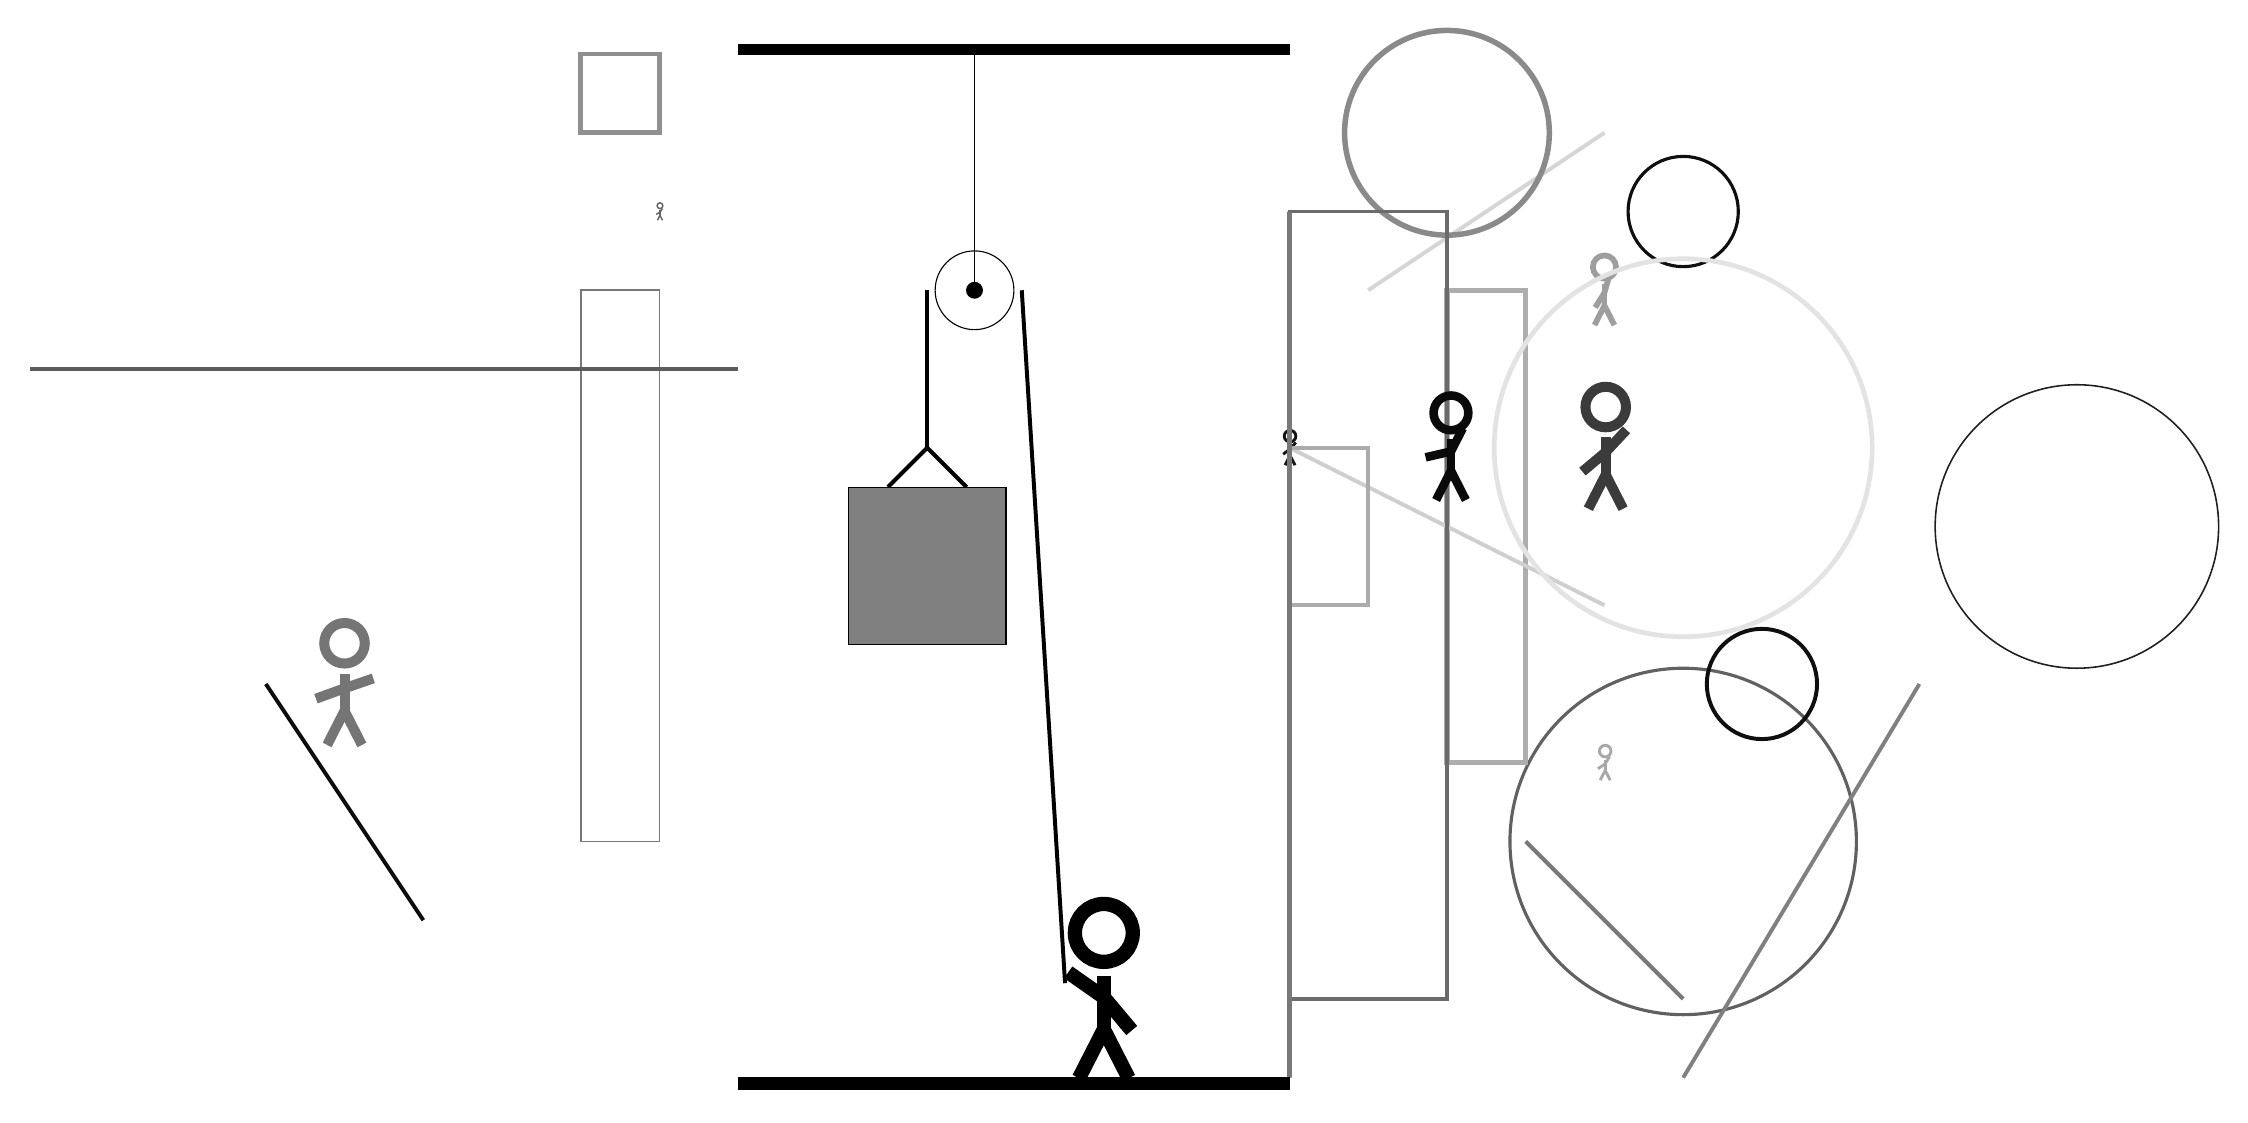
\begin{tikzpicture}
		%%%%% START %%%%%
		
		\draw[fill=black] (-2, 10) rectangle (5, 10.125);
		
		\draw (1, 7) circle (0.5);
		\draw[fill=black] (1, 7) circle (0.1);
		\draw (1, 10) -- (1, 7);
		
		\draw [line width=0.4mm, color=black!62](10, 0) circle (2.2);
		
		\node[line width=0.2mm, color=black!92] at (5, 5) {\Strichmaxerl[2][37][48]};
		\draw[line width=0.5mm, color=black!16](6, 7) -- (9, 9);
		\node[line width=0.4mm, color=black!34] at (9, 1) {\Strichmaxerl[2][33][60]};
		
		\draw [line width=0.5mm, color=black!94](11, 2) circle (0.7);
		\draw [line width=0.7mm, color=black!46](7, 9) circle (1.3);
		\node[line width=0.4mm, color=black!77] at (9, 5) {\Strichmaxerl[7][40][47]};
		\draw [line width=0.4mm, color=black!94](10, 8) circle (0.7);
		\draw[line width=0.5mm, color=black!95](-6, -1) -- (-8, 2);
		\draw[line width=0.6mm, color=black!44] (-4, 9) rectangle (-3, 10);
		\draw[line width=0.7mm, color=black!32] (7, 7) rectangle (8, 1);
		
		\node[line width=0.3mm, color=black!54] at (-7, 2) {\Strichmaxerl[7][20][19]};
		\draw[line width=0.5mm, color=black!19](5, 5) -- (9, 3);
		
		\draw[line width=0.5mm, color=black!52](8, 0) -- (10, -2);
		\draw[line width=0.5mm, color=black!50](10, -3) -- (13, 2);
		\draw[line width=0.5mm, color=black!33] (6, 3) rectangle (5, 5);
		
		\node[line width=0.2mm, color=black!38] at (9, 7) {\Strichmaxerl[4][58][74]};
		
		\node[line width=0.7mm, color=black!62] at (-3, 8) {\Strichmaxerl[1][31][55]};
		\draw [line width=0.6mm, color=black!11](10, 5) circle (2.4);
		\draw [line width=0.2mm, color=black!88](15, 4) circle (1.8);
		\draw[line width=0.2mm, color=black!53] (-4, 0) rectangle (-3, 7);
		\draw[line width=0.5mm, color=black!58] (7, 8) rectangle (5, -2);
		\draw[line width=0.5mm, color=black!64](-2, 6) -- (-11, 6);
		\draw[line width=0.7mm, color=black!53] (5, 8) rectangle (5, -3);
		\node[line width=0.7mm, color=black!96] at (7, 5) {\Strichmaxerl[6][13][63]};
		
		
		\draw[line width=0.5mm] (-0.1, 4.5) -- (0.4, 5.0) -- (0.9, 4.5);
		\draw[fill=black!50] (-0.6, 4.5) rectangle (1.4, 2.5);
		
		\draw[line width=0.5mm] (0.4, 7) -- (0.4, 5.0);
		\centerarc[line width=0.5mm](1, 7)(0:180:0.6);
		\draw[line width=0.5mm](1.6, 7) -- (2.15, -1.8);
		
		\node at (2.6, -1.9) {\Strichmaxerl[10][-35][-50]};
		
		\draw[fill=black] (-2, -3) rectangle (5, -3.15);
		
		%%%%% END %%%%%
	\end{tikzpicture}
\end{document}